%%%%%%%%%%%%%%%%%%%%%%%%%%%%%%%%%%%%%%%%%
% Beamer Presentation
% LaTeX Template
% Version 1.0 (10/11/12)
%
% This template has been downloaded from:
% http://www.LaTeXTemplates.com
%
% License:
% CC BY-NC-SA 3.0 (http://creativecommons.org/licenses/by-nc-sa/3.0/)
%
%%%%%%%%%%%%%%%%%%%%%%%%%%%%%%%%%%%%%%%%%

%----------------------------------------------------------------------------------------
%	PACKAGES AND THEMES
%----------------------------------------------------------------------------------------

\documentclass{beamer}

\mode<presentation> {

% The Beamer class comes with a number of default slide themes
% which change the colors and layouts of slides. Below this is a list
% of all the themes, uncomment each in turn to see what they look like.

%\usetheme{default}
%\usetheme{AnnArbor}
%\usetheme{Antibes}
%\usetheme{Bergen}
%\usetheme{Berkeley}
%\usetheme{Berlin}
%\usetheme{Boadilla}
%\usetheme{CambridgeUS}
%\usetheme{Copenhagen}
%\usetheme{Darmstadt}
%\usetheme{Dresden}
%\usetheme{Frankfurt}
%\usetheme{Goettingen}
%\usetheme{Hannover}
%\usetheme{Ilmenau}
%\usetheme{JuanLesPins}
%\usetheme{Luebeck}
\usetheme{Madrid}
%\usetheme{Malmoe}
%\usetheme{Marburg}
%\usetheme{Montpellier}
%\usetheme{PaloAlto}
%\usetheme{Pittsburgh}
%\usetheme{Rochester}
%\usetheme{Singapore}
%\usetheme{Szeged}
%\usetheme{Warsaw}

% As well as themes, the Beamer class has a number of color themes
% for any slide theme. Uncomment each of these in turn to see how it
% changes the colors of your current slide theme.

%\usecolortheme{albatross}
%\usecolortheme{beaver}
%\usecolortheme{beetle}
%\usecolortheme{crane}
%\usecolortheme{dolphin}
%\usecolortheme{dove}
%\usecolortheme{fly}
%\usecolortheme{lily}
%\usecolortheme{orchid}
%\usecolortheme{rose}
%\usecolortheme{seagull}
%\usecolortheme{seahorse}
%\usecolortheme{whale}
%\usecolortheme{wolverine}

%\setbeamertemplate{footline} % To remove the footer line in all slides uncomment this line
%\setbeamertemplate{footline}[page number] % To replace the footer line in all slides with a simple slide count uncomment this line

%\setbeamertemplate{navigation symbols}{} % To remove the navigation symbols from the bottom of all slides uncomment this line
}

\usepackage{graphicx} % Allows including images
\usepackage{booktabs} % Allows the use of \toprule, \midrule and \bottomrule in tables
\usepackage{multirow}
\usepackage{adjustbox}
\usepackage{array}
\usepackage{tikz}
\usepackage{soul}
\usepackage{pdfpages}
\usetikzlibrary{shapes.geometric, arrows, positioning, fit}
\usepackage[latin1]{inputenc}
\newcommand{\xmark}{\textcolor{red}{\text{\sffamily X}}}
\newcommand{\cmark}{\textcolor{green}{\checkmark}}
\newcommand{\tr}{\text{tr}}
\newcommand{\E}{\textbf{E}}
\newcommand{\diag}{\text{diag}}
\newcommand{\argmax}{\text{argmax}}
\newcommand{\argmin}{\text{argmin}}
\newcommand{\Cov}{\text{Cov}}
\newcommand{\Var}{\text{Var}}
\newcommand{\Vol}{\text{Vol}}
\newcommand{\bx}{\boldsymbol{x}}
\newcommand{\by}{\boldsymbol{y}}
\newcommand{\bX}{\boldsymbol{X}}
\newcommand{\bY}{\boldsymbol{Y}}
\sethlcolor{gray}
\makeatletter
\newcommand\SoulColor{%
  \let\set@color\beamerorig@set@color
  \let\reset@color\beamerorig@reset@color}
\makeatother
\definecolor{color1}{RGB}{128,13,13}
\definecolor{color2}{RGB}{70,128,13}
\definecolor{color3}{RGB}{13,128,128}
\definecolor{color4}{RGB}{70,13,128}

%tikz stufff


%----------------------------------------------------------------------------------------
%	TITLE PAGE
%----------------------------------------------------------------------------------------


\title[tfMRI generalizability]{Using randomization in fMRI classification experiments to ensure generalizability}

\author{Charles Zheng} % Your name
\institute[NIMH] % Your institution as it will appear on the bottom of every slide, may be shorthand to save space
{National Institute of Mental Health}
\date{\today} % Date, can be changed to a custom date

\begin{document}

\begin{frame}
\titlepage % Print the title page as the first slide
(Joint work with Yuval Benjamini.)
\end{frame}

\section{Randomization and Generalization}

\begin{frame}
\frametitle{Reproducibility}
\begin{center}
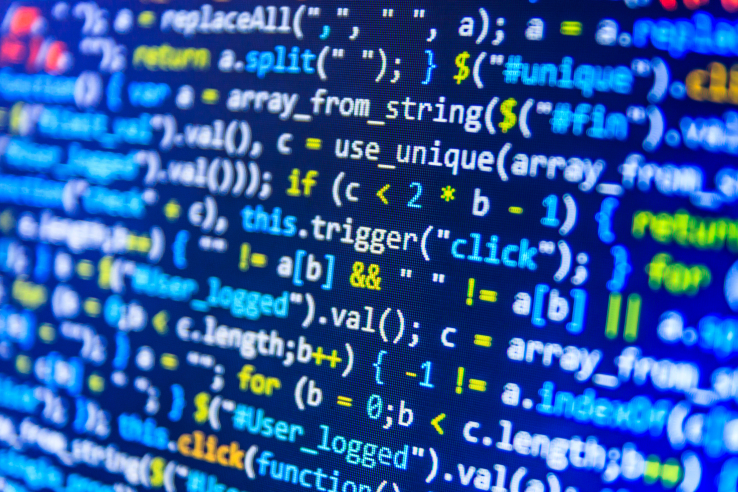
\includegraphics[scale = 0.8]{code_clipart.jpg}
\end{center}
Transparency in sharing data, methods, code, etc.
\end{frame}

\begin{frame}
\frametitle{Replicability}
\begin{center}
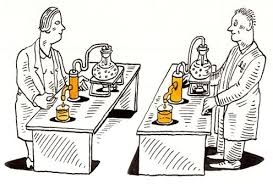
\includegraphics[scale = 0.7]{replicability.jpg} 
\end{center}
``The ability of a researcher to duplicate the results of a prior
study if the same procedures are followed but new data are
collected''--National Science Foundation
\end{frame}

\begin{frame}
\frametitle{Generalizability}
\begin{center}
\begin{tabular}{ccc}
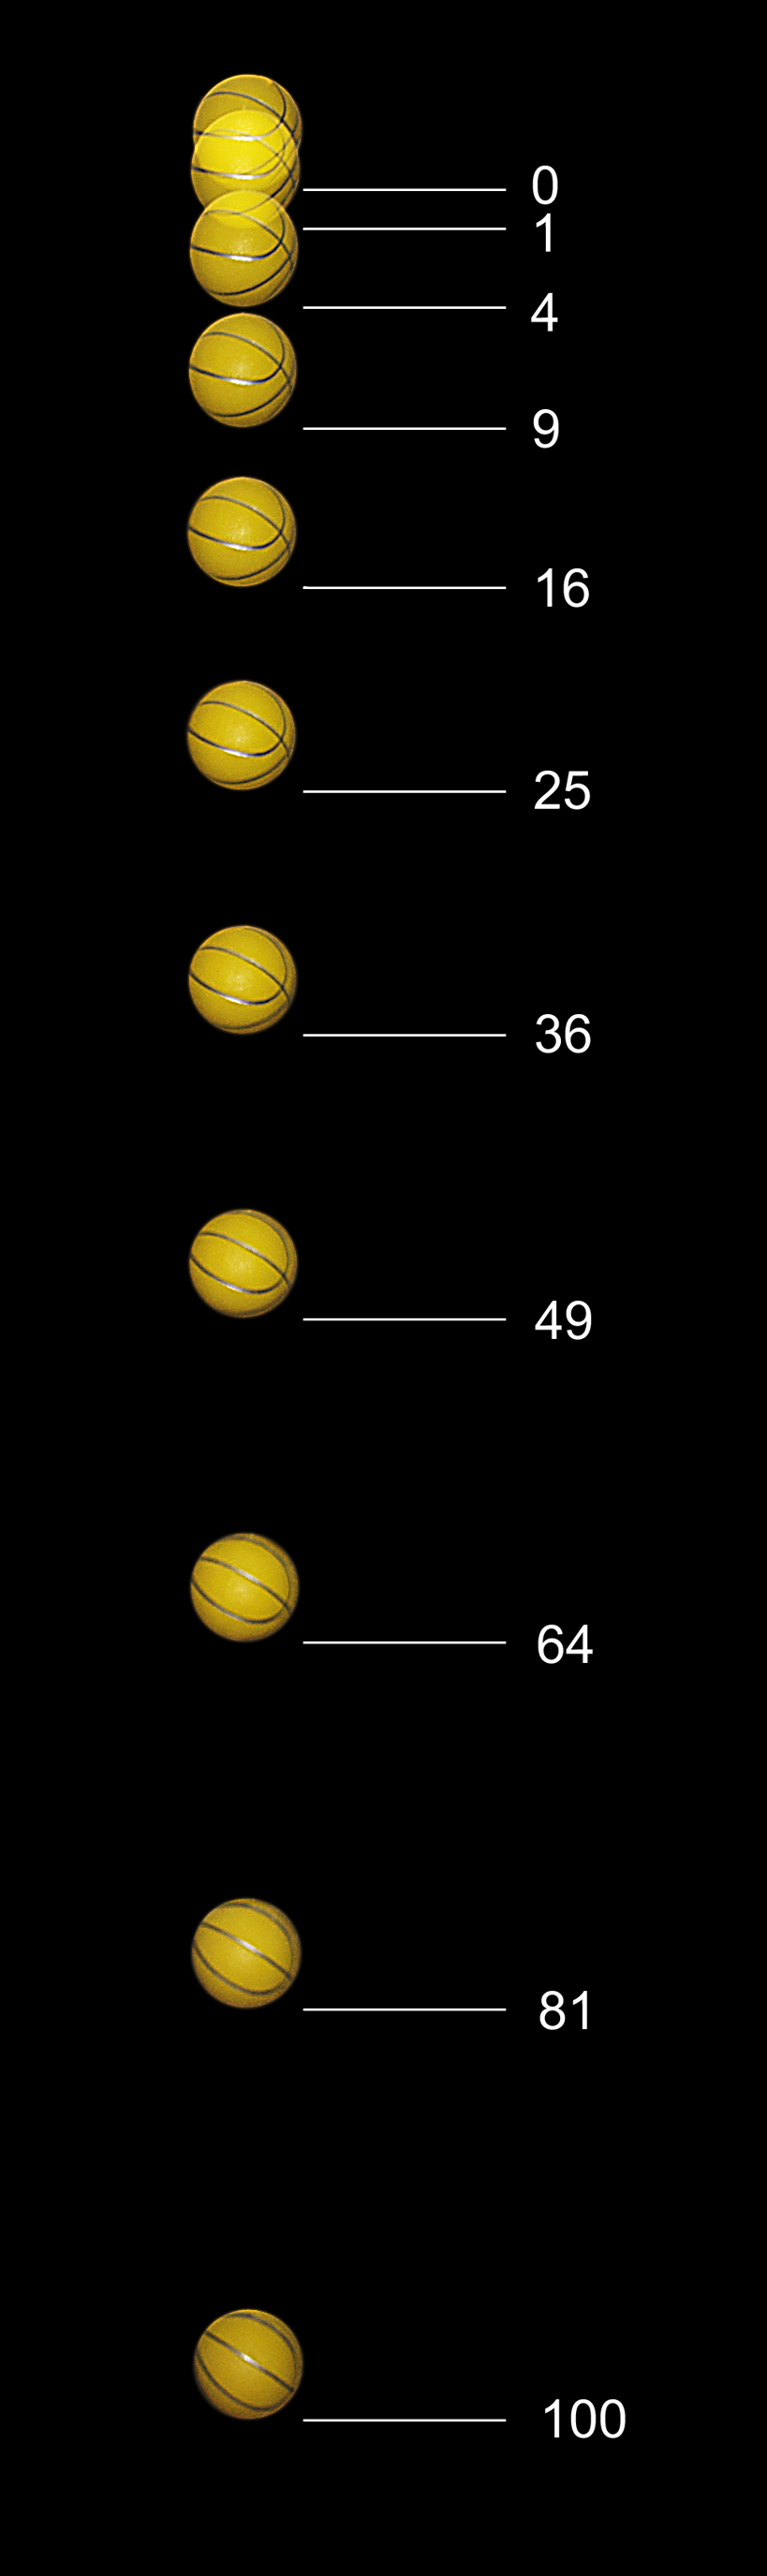
\includegraphics[scale = 0.1]{Falling_ball.jpg} &
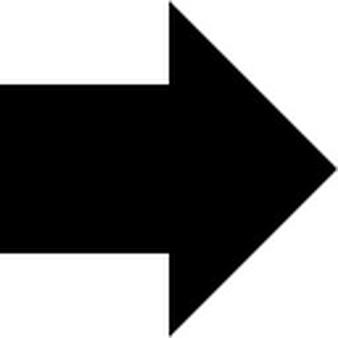
\includegraphics[scale = 0.3]{right_arrow.jpg} &
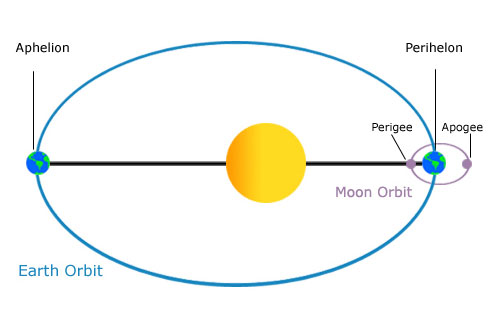
\includegraphics[scale = 0.3]{orbit-3.jpg} 
\end{tabular}
\end{center}
Being able to predict results of new ``experiments'' or observations.
\end{frame}

\begin{frame}
\frametitle{Problem of Induction}
\begin{center}
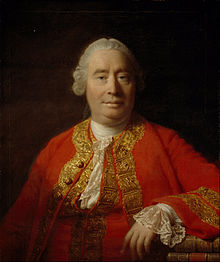
\includegraphics[scale = 0.6]{david_hume.jpg}

David Hume (1711-1776)
\end{center}
Why is it that ``instances of which we have had no experience resemble
those of which we have had experience''?
\end{frame}

\begin{frame}
\frametitle{Peirceian Induction and Neyman-Pearson testing}
\begin{center}
\begin{tabular}{cc}
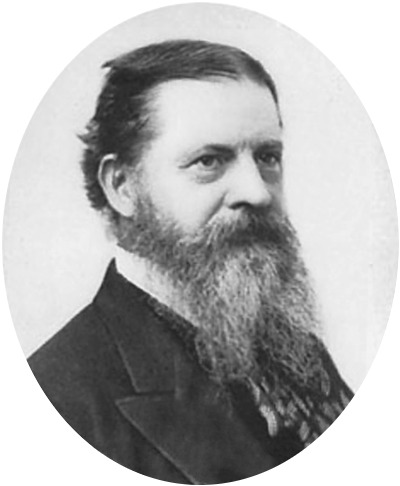
\includegraphics[scale = 0.3]{peirce.jpg} &
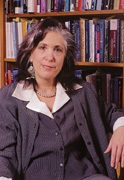
\includegraphics[scale = 0.8]{dmayo1.jpg} \\
C. S. Pierce & Deborah Mayo
\end{tabular}
\end{center}
Theories can be confirmed inductively via \emph{severe testing}.  The Neyman-Pearson (classical statistical) framework provides one such mechanism.
\end{frame}

\begin{frame}
\frametitle{Generalizing from samples to population}
\begin{center}
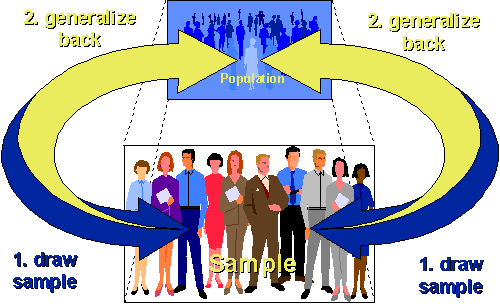
\includegraphics[scale = 0.3]{extsamp.png}
\end{center}
Thanks to key results in probability theory (law of large numbers, central limit theorem), sampling from a defined population is a well-understood form of induction.
\end{frame}

\begin{frame}
\frametitle{Randomized Experiments enable Generalization}
\begin{center}
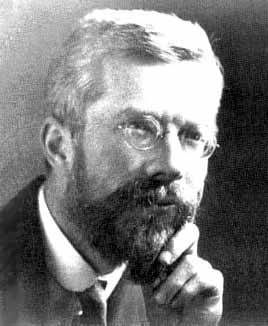
\includegraphics[scale = 0.3]{RA_Fisher.jpg}
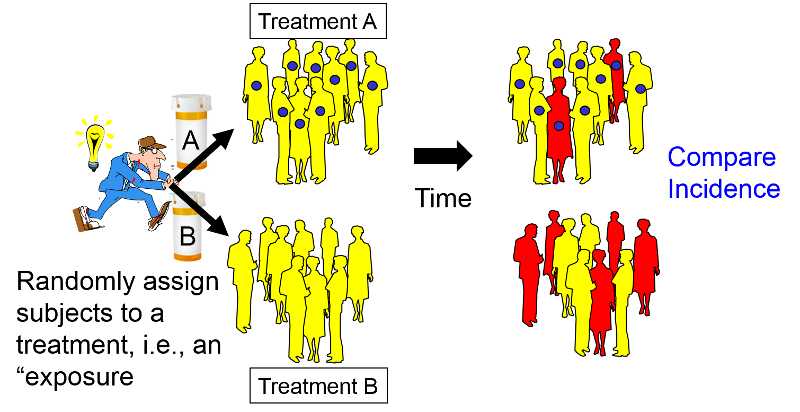
\includegraphics[scale = 0.2]{RCT_Cartoon.png}
\end{center}
\begin{itemize}
\item \emph{Design of Experiments} by R. A. Fisher introduced the concept of \emph{randomization}
\item \emph{Randomized clinical trials} are the gold standard
for inference of causal effects.
\item Randomization + Law of Large Numbers implies quantitative replicability--a form of generalization to the population
\end{itemize}
\end{frame}

\begin{frame}
\frametitle{Random vs deterministic design in fMRI}
For designing event-related sequences for task fMRI...
\begin{itemize}
\item Bura\v{c}as and Boynton (2001) showed that deterministic m-sequences are more efficient for estimating HRF than random designs by a large factor
\begin{center}
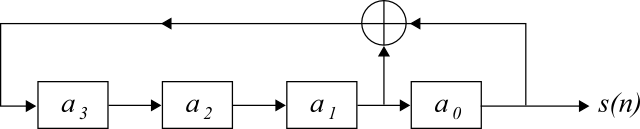
\includegraphics[scale = 0.2]{MLS_shiftregisters_L4.png}
\end{center}
\item However, as Friston (1999) points out, random designs may have advanatages in terms of psychological effects
\item Theoretically speaking, deterministic designs are fine as long as one can rule out higher-order dependencies between measurements
\item However, when no principled approach exists to cancel out possible biases, randomization guarantees it (on average)
\end{itemize}
\end{frame}

\begin{frame}
\frametitle{Generalizing beyond the population?}
\begin{center}
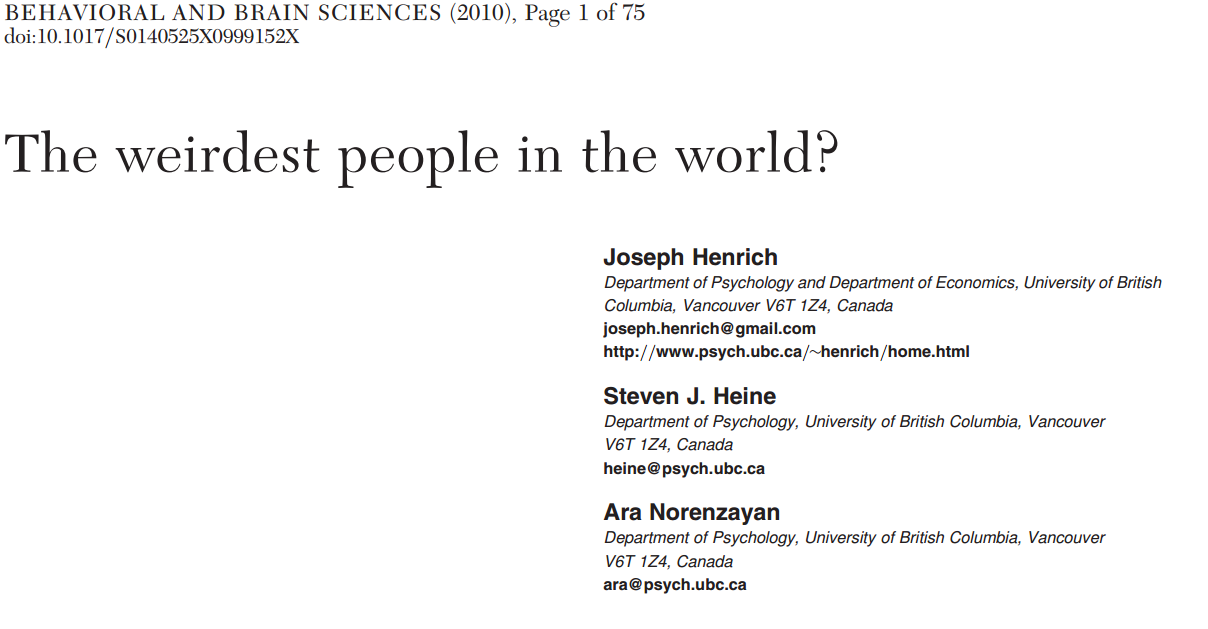
\includegraphics[scale = 0.3]{weird_people.png}
\end{center}
\end{frame}


\section{Classification experiments in fMRI}

\begin{frame}
\sectionpage
\end{frame}

\begin{frame}
\frametitle{Studying the neural code}
\begin{center}
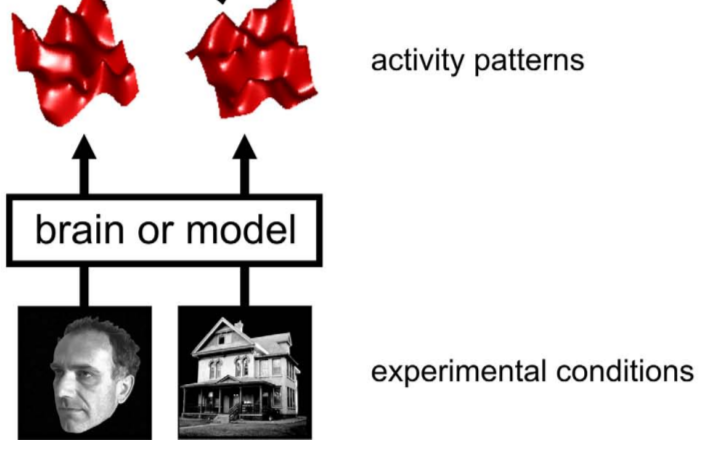
\includegraphics[scale = 0.3]{k08_step1.png}
\end{center}
Present the subject with visual stimuli, pictures of faces and houses.
Record the subject's brain activity in the fMRI scanner.
\end{frame}

%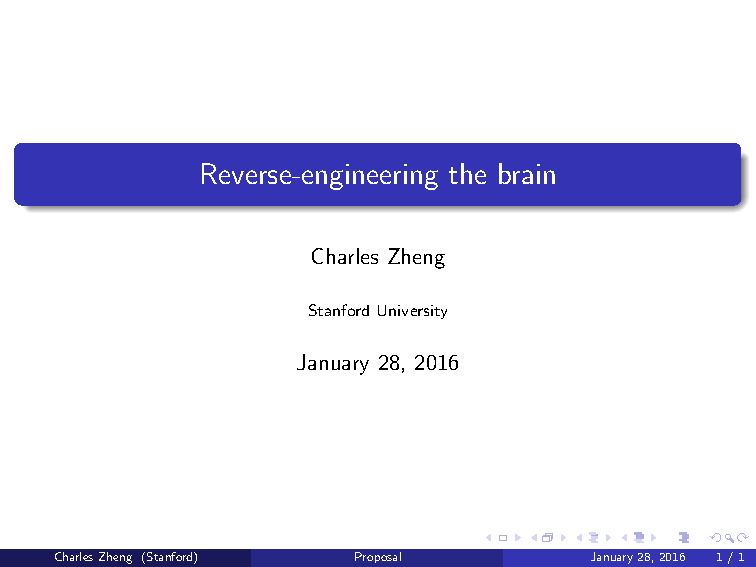
\includepdf[pages=1]{Zheng_proposal.pdf}
{
\setbeamercolor{background canvas}{bg=}
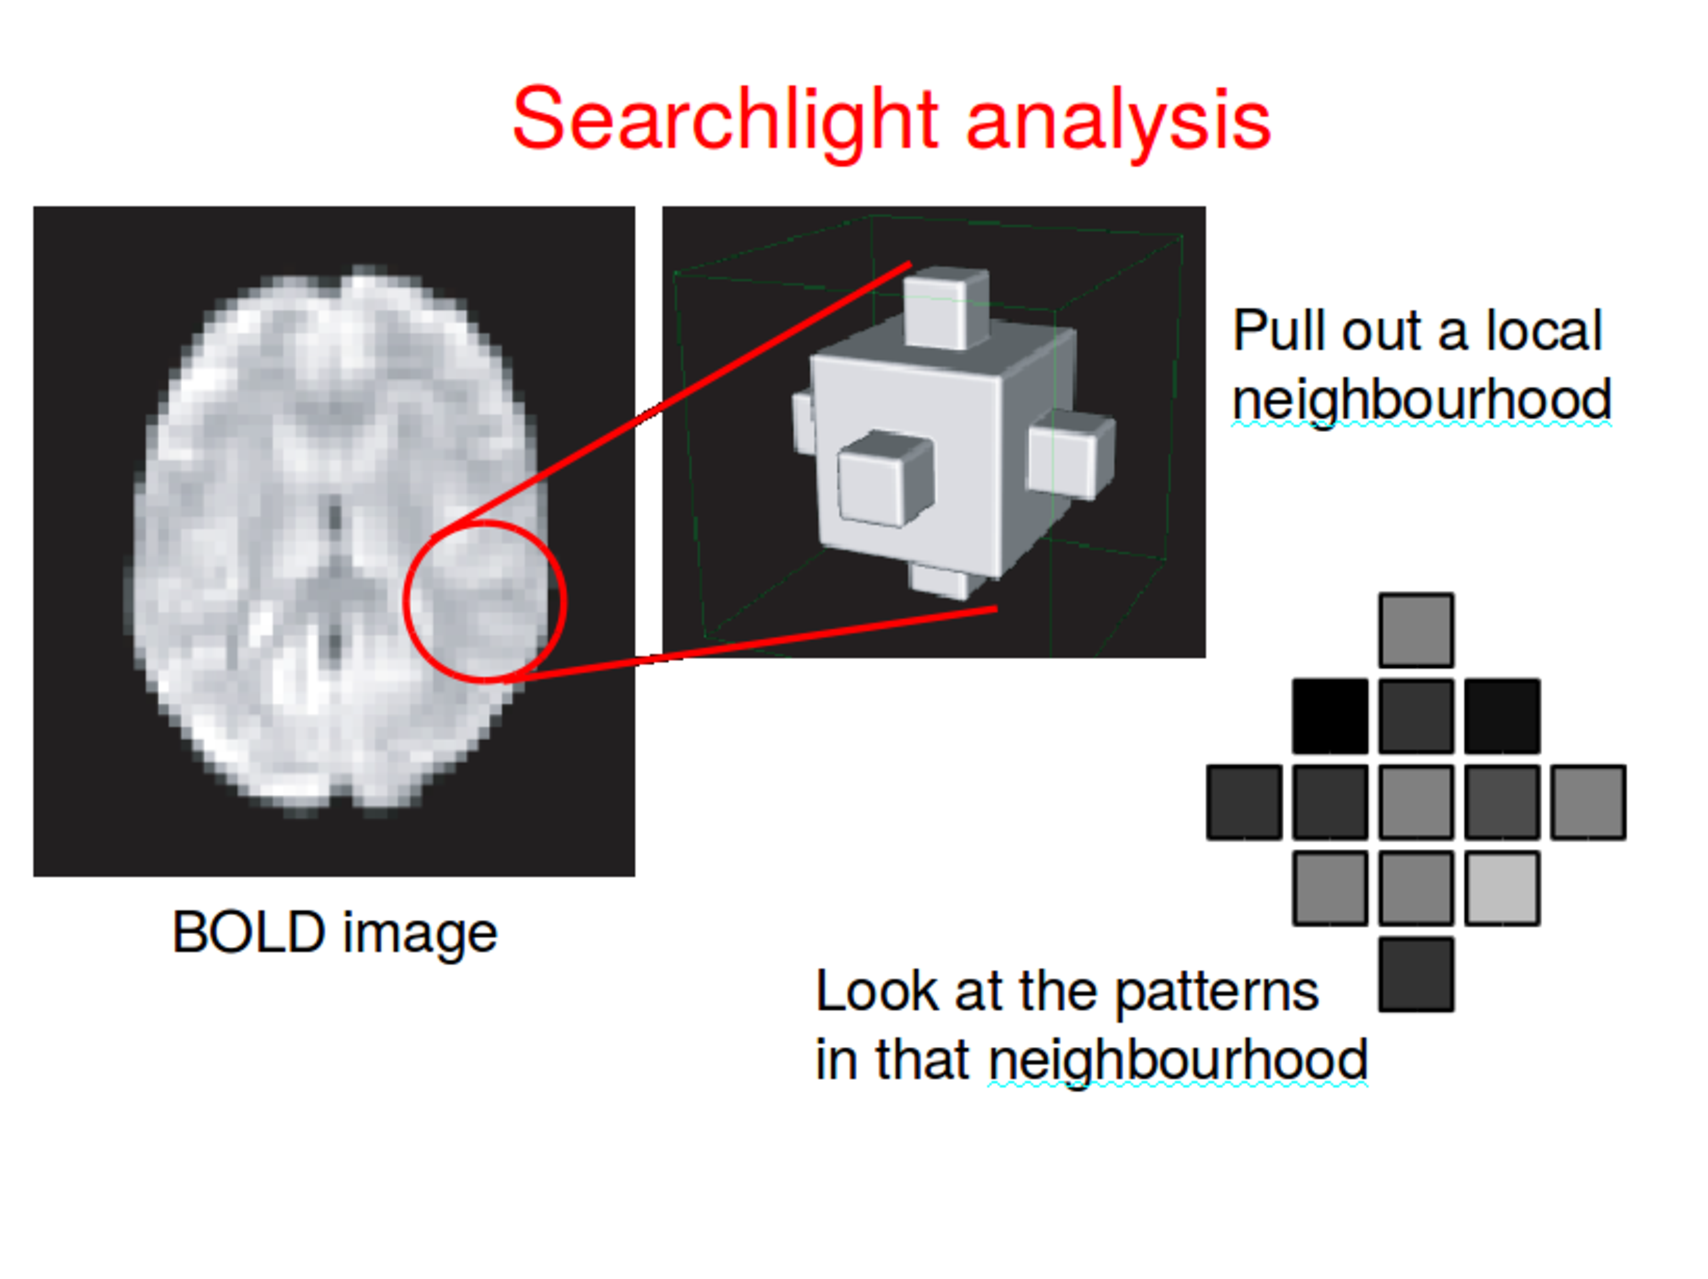
\includepdf[pages=1]{searchlight_slide.pdf}
% from Razaida
}

\begin{frame}
\frametitle{Searchlight analysis}
\begin{center}
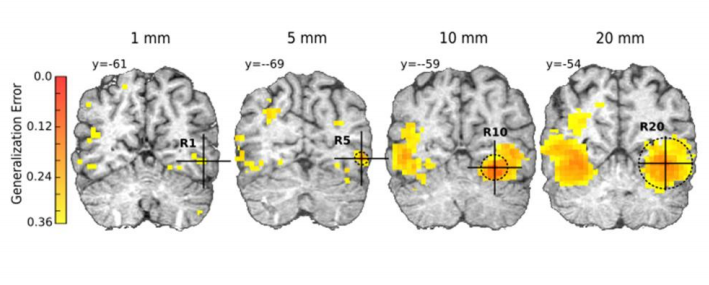
\includegraphics[scale = 0.5]{searchlight_windowsize.png}
\end{center}
Produces a map of ``informative'' regions of the brain (as measured by generalization accuracy).
\end{frame}

{
\setbeamercolor{background canvas}{bg=}
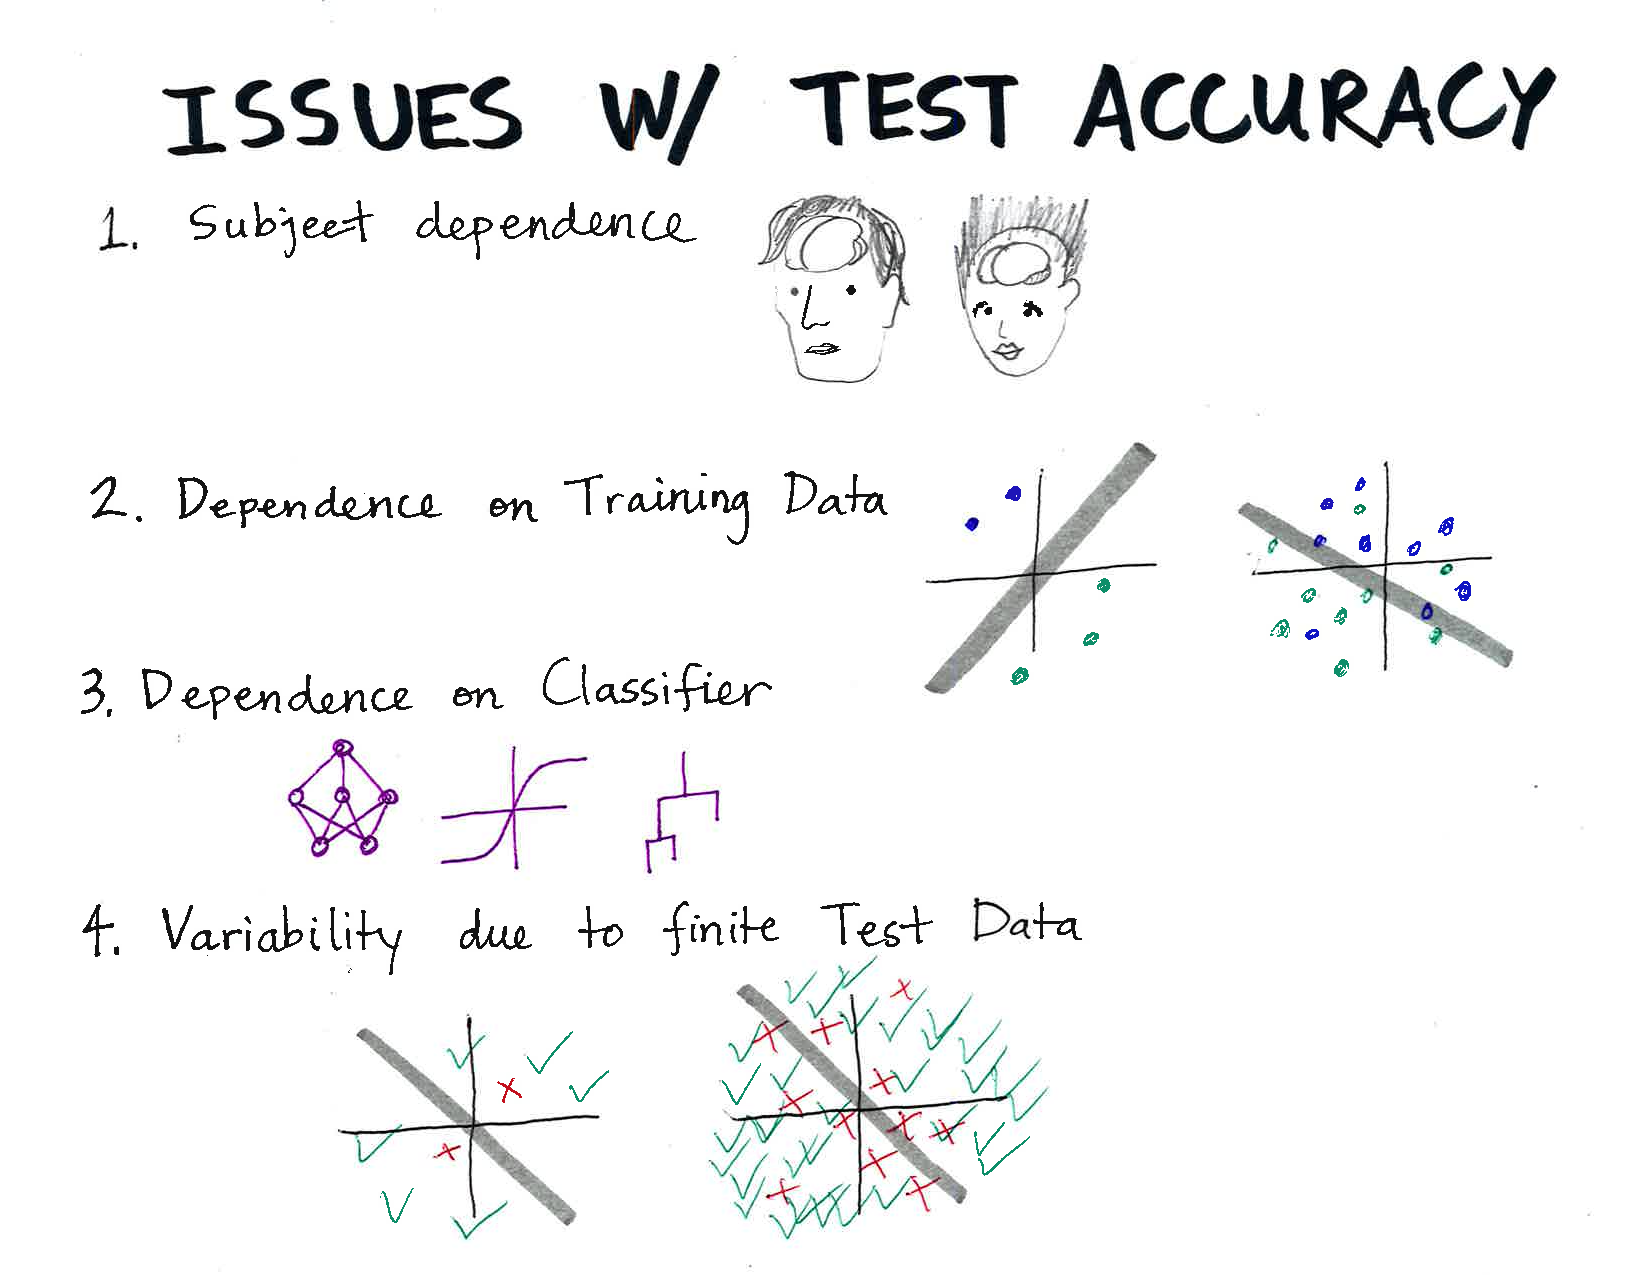
\includepdf[pages=1-2]{drawings_einstein.pdf}
% from Razaida
}

\begin{frame}
\frametitle{Bayes accuracy}
\begin{itemize}
\item Discrete $Y \in \{1,...,k\}$, continuous or discrete $X$.
\item A classifier is a function $f$ mapping $x$ to a label in $\{1,..,k\}$
\item Generalization accuracy of the classifier:
\[
\text{GA}(f) = \Pr[Y = f(x)]
\]
\item Bayes accuracy:
\[
\text{BA} = \sup_f \Pr[Y = f(x)] = \Pr[Y = \text{argmax}_{i=1} p(X|Y=i)]
\]
\item Since random guessing is correct with probability $1/k$,
\[
\text{BA} \in [1/k, 1]
\]
(if $Y$ is uniformly distributed)
\end{itemize}
\end{frame}

\begin{frame}
\frametitle{Fixed classification task}
\begin{columns}
\begin{column}{0.6\textwidth}
\begin{tabular}{cc}
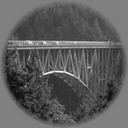
\includegraphics[scale = 0.5]{img1.png} &
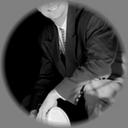
\includegraphics[scale = 0.5]{img2.png} \\
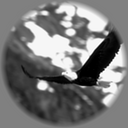
\includegraphics[scale = 0.5]{img3.png} &
\end{tabular}
\end{column}
\begin{column}{0.4\textwidth}
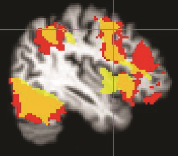
\includegraphics[scale = 0.5]{smbrain1.png}
\end{column}
\end{columns}
\begin{itemize}
\item Different stimuli sets lead to different \emph{Bayes accuracy}.
\end{itemize}
\end{frame}

\begin{frame}
\frametitle{Fixed classification task}
\begin{columns}
\begin{column}{0.6\textwidth}
\begin{tabular}{cc}
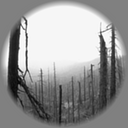
\includegraphics[scale = 0.5]{img5.png} &
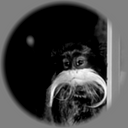
\includegraphics[scale = 0.5]{img6.png} \\
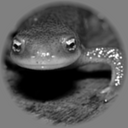
\includegraphics[scale = 0.5]{img7.png} &
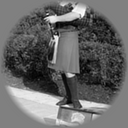
\includegraphics[scale = 0.5]{img8.png}
\end{tabular}
\end{column}
\begin{column}{0.4\textwidth}
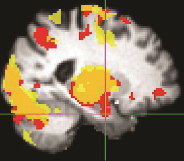
\includegraphics[scale = 0.5]{smbrain2.png}
\end{column}
\end{columns}
\begin{itemize}
\item Different stimuli sets lead to different \emph{Bayes accuracy}.
\item Results are incomparable, even in the large-sample limit.
\end{itemize}
\end{frame}

\begin{frame}
\frametitle{Generalizing beyond the design}

\begin{columns}
\begin{column}{0.6\textwidth}
\begin{center}
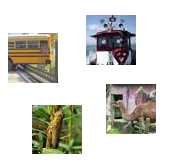
\includegraphics[scale = 1]{imagenet_sub.png}
\end{center}
\end{column}
\begin{column}{0.4\textwidth}
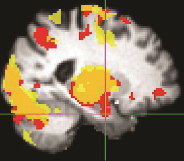
\includegraphics[scale = 0.5]{smbrain2.png}
\end{column}
\end{columns}

Scientists are not innately interested in the Bayes accuracy of a \emph{particular} stimuli set, which is often chosen arbitrarily...

\end{frame}

\begin{frame}
\frametitle{Generalizing beyond the design}

\begin{columns}
\begin{column}{0.6\textwidth}
\begin{center}
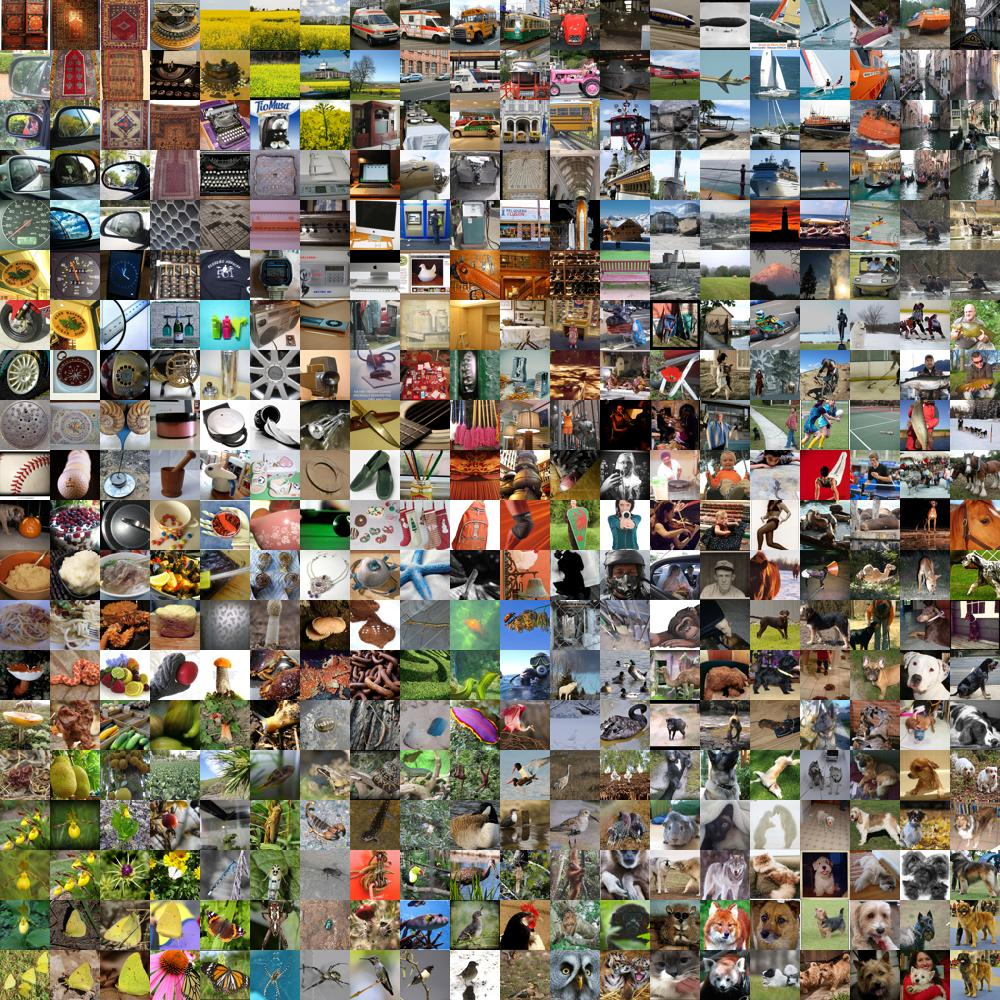
\includegraphics[scale = 0.1]{imagenet.jpg}
\end{center}
\end{column}
\begin{column}{0.4\textwidth}
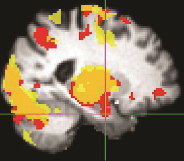
\includegraphics[scale = 0.5]{smbrain2.png}
\end{column}
\end{columns}
\vspace{0.2in}
But it would be more interesting to be able to make inferences from the data about a \emph{larger} class of stimuli...

\end{frame}

\section{Randomized classification and Average Bayes accuracy}

\begin{frame}
\sectionpage
\end{frame}

\begin{frame}
\frametitle{Randomized classification}
\begin{tabular}{c|c|c}
1. Population of stimuli $p(x)$ & 
2. Subsample $k$ stimuli &
3. Data\\
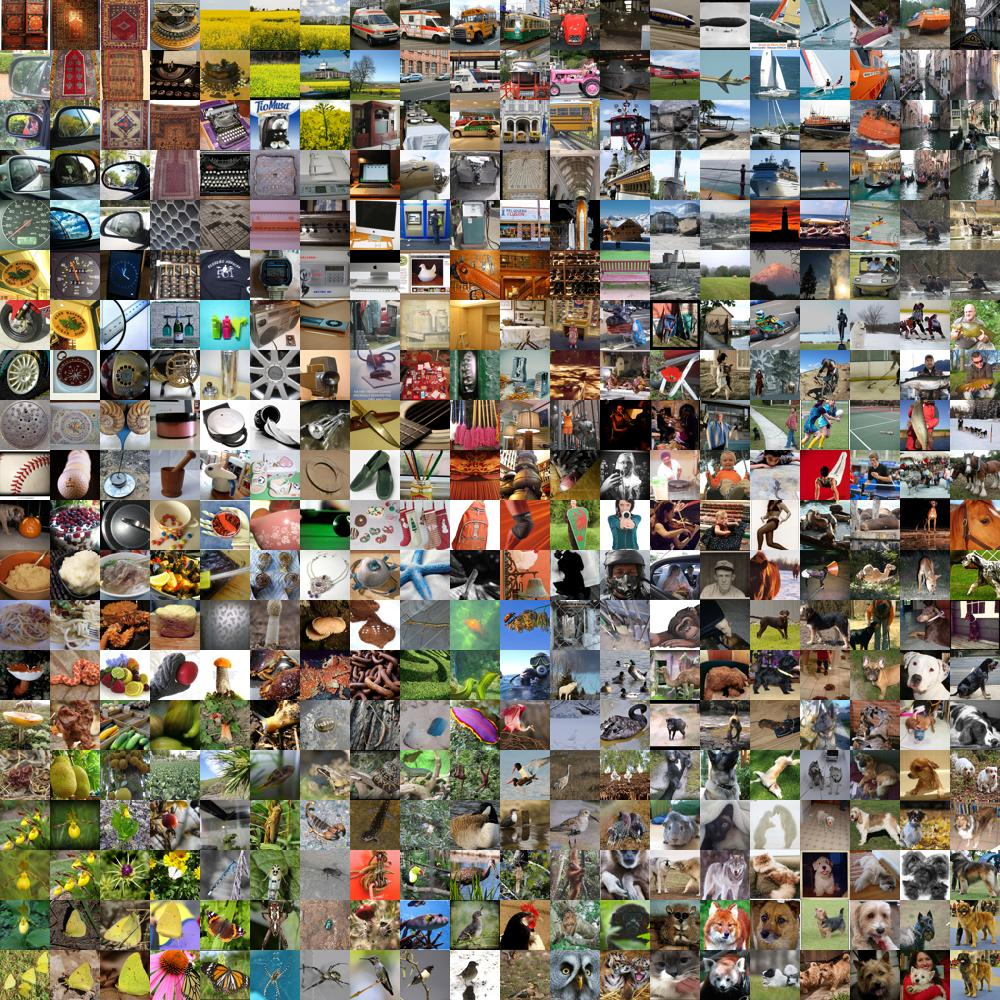
\includegraphics[scale = 0.05]{imagenet.jpg} &
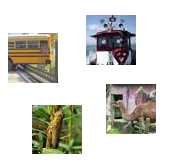
\includegraphics[scale = 0.5]{imagenet_sub.png} &
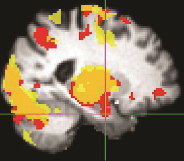
\includegraphics[scale = 0.3]{smbrain2.png}
\end{tabular}

\vspace{0.2in}
4. Train a classifier

\vspace{0.2in}
5. Estimate generalization accuracy (which is lower bound for the \emph{random} Bayes accuracy $\text{BA}_k$)
\end{frame}

\begin{frame}
\frametitle{Average Bayes accuracy}
\begin{center}
\begin{tabular}{c|c|c|c}
& Experiment 1 & Experiment 2 & Experiment 3\\\hline
&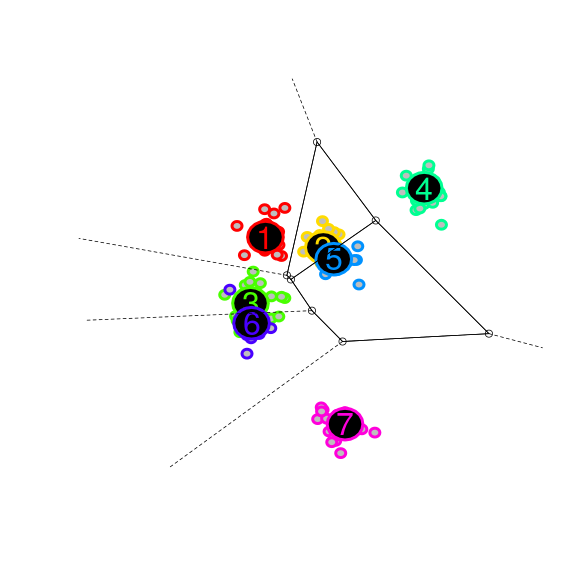
\includegraphics[scale = 0.15, clip = true, trim = 0.6in 0.2in 0.6in 0.2in]{../info_theory_paper/gaussian_figure1a.png} &
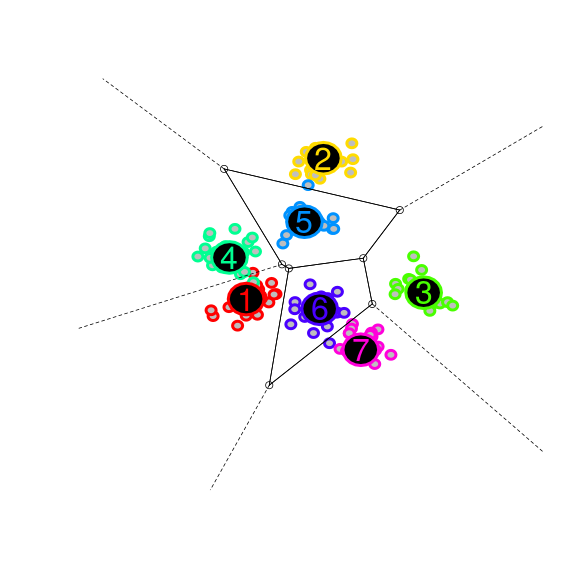
\includegraphics[scale = 0.15, clip = true, trim = 0.6in 0.2in 0.6in 0.2in]{../info_theory_paper/gaussian_figure1b.png} &
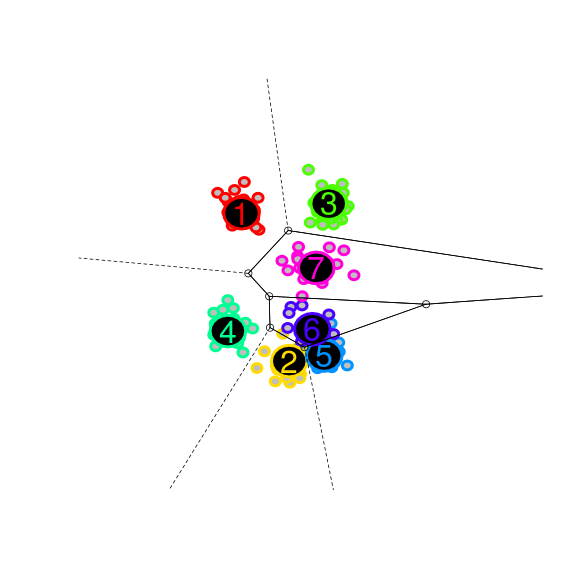
\includegraphics[scale = 0.15, clip = true, trim = 0.6in 0.2in 0.6in 0.2in]{../info_theory_paper/gaussian_figure1c.png}\\\hline
Bayes accuracy & 0.55 & 0.65 & 0.52 \\
\end{tabular}
\end{center}
\begin{itemize}
\item Bayes accuracy depends on the stimuli drawn.
\item Therefore, define $k$-class \emph{average Bayes accuracy} as the expected Bayes accuracy for $X_1,..,X_k \stackrel{iid}{\sim} p(x)$.
\[
\text{ABA}_k = \E[BA(X_1,...,X_k)]
\]
\end{itemize}
\end{frame}

\begin{frame}
\frametitle{Average Bayes accuracy}
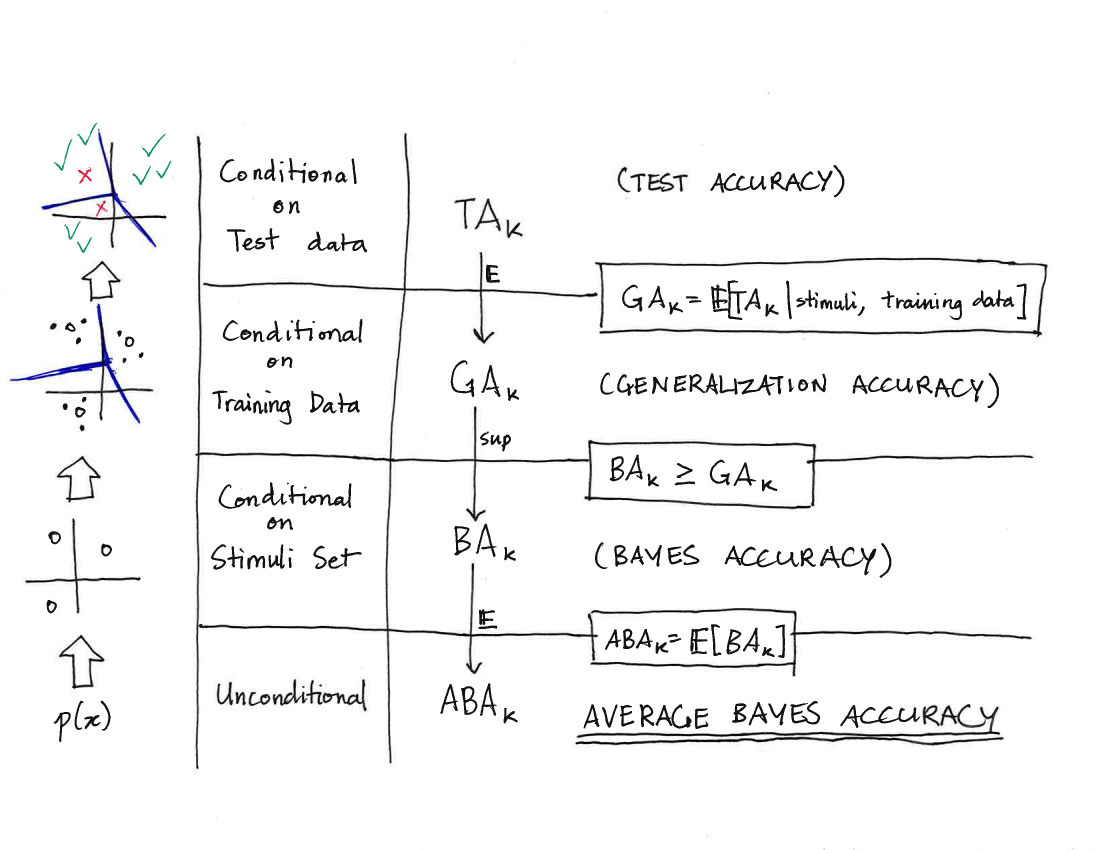
\includegraphics[scale = 0.45, clip = true, trim = 0in 1in 0.5in 1in]{ta_to_aba.png}
\end{frame}

\begin{frame}
\frametitle{Inferring average Bayes accuracy}

\begin{itemize}
\item $\text{BA}_k \stackrel{def}{=} \text{BA}(X_1,..,X_k)$ is unbiased estimate of
\[
\text{ABA}_k = \E[BA_k]
\]
by definition.
\item But what is the variance?
\[
\text{Var}[\text{BA}(X_1,...,X_k)]
\]
\item \emph{Theoretical result}. Maximal variability is of order $1/k$.
\item Therefore, it is feasbile to get a good idea of $\text{ABA}_k$ by choosing a sufficiently large sample size $k$.
\end{itemize}
\end{frame}

\begin{frame}
\frametitle{Two intuitions for variability result}
Why does variability decrease with $k$?
\begin{itemize}
\item 1. Bayes accuracy behaves like an average of $k$ i.i.d random variables. (Also gives correct $1/k$ rate.)
\item 2. Bayes accuracy behaves like a max of $k$ i.i.d. random variables.
\end{itemize}
\end{frame}

\begin{frame}
\frametitle{Intuition 1: averaging}
\begin{center}
\begin{tabular}{c|c|c|c}
& Experiment 1 & Experiment 2 & Experiment 3\\\hline
&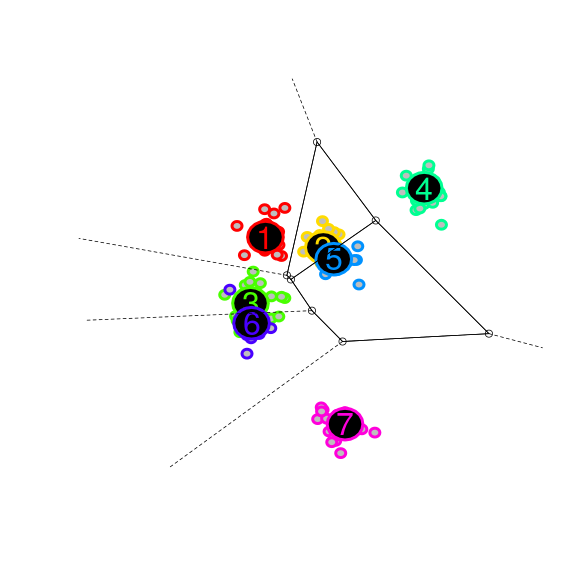
\includegraphics[scale = 0.15, clip = true, trim = 0.6in 0.2in 0.6in 0.2in]{../info_theory_paper/gaussian_figure1a.png} &
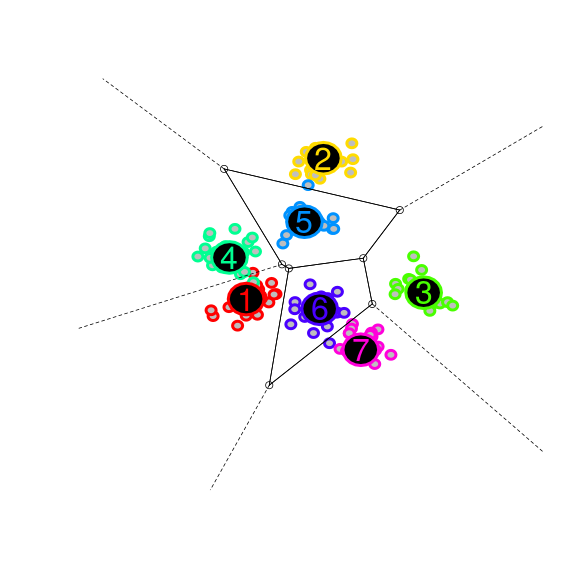
\includegraphics[scale = 0.15, clip = true, trim = 0.6in 0.2in 0.6in 0.2in]{../info_theory_paper/gaussian_figure1b.png} &
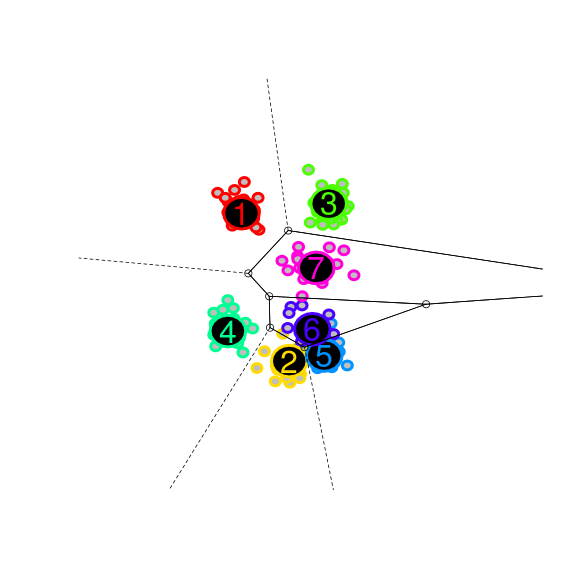
\includegraphics[scale = 0.15, clip = true, trim = 0.6in 0.2in 0.6in 0.2in]{../info_theory_paper/gaussian_figure1c.png}\\\hline
Bayes accuracy & 0.55 & 0.65 & 0.52 \\
\end{tabular}
\end{center}
Average of $k$ gaussian probability integrals... (which are asympt. uncorrelated.)
\end{frame}

\begin{frame}
\frametitle{Intuition 2: An identity}
\begin{itemize}
\item It is a well-known result from Bayesian inference that the optimal classifier $f$ is defined as
\[
f(y) = \text{argmax}_{i=1}^k p(y|x_i),
\]
since the prior class probabilities are uniform.
\item Therefore,
\begin{align*}
\text{BA}(x_1,...,x_k) &= \Pr[\text{argmax}_{i=1}^k p(y|x_i) = Z| x_1,...,x_k] 
\\&= \frac{1}{k}\int \max_{i=1}^k p(y|x_i) dy.
\end{align*}
\end{itemize}
\end{frame}

\begin{frame}
\frametitle{Intuition behind identity}
\begin{columns}
\begin{column}{0.5\textwidth}
\begin{center}
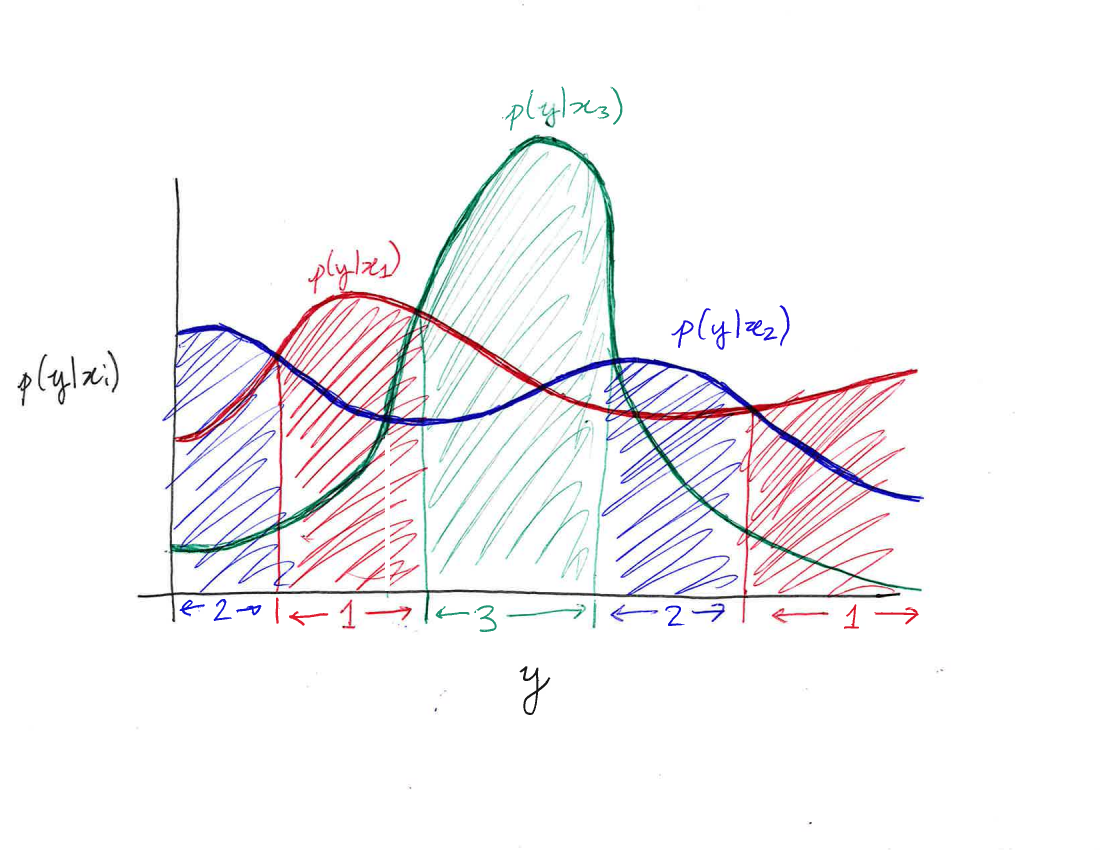
\includegraphics[scale = 0.35, clip = true, trim = 1.2in 1.3in 0in 1in]{var_ba.png}
\end{center}   
\end{column}
\begin{column}{0.5\textwidth}  %%<--- here
\begin{align*}
\text{BA}&(x_1,x_2,x_3) \\&= \sum_i \Pr[x_i]\Pr_{Y \sim p(y|x_i)}[Y \in \text{zone }i]
\\&= \sum_i \frac{1}{k} \text{Area under curve $i$ in zone $i$}
\\&\ \ \ = \frac{1}{k} \text{Area under } \max_{i=1}^k p(y|x_i)
\end{align*}
\end{column}
\end{columns}
\end{frame}

\begin{frame}
\frametitle{Variability of Bayes accuracy}

\emph{Theoretical result}. In the max formulation of $\text{BA}_k$, we
can apply Efron-Stein inequality to get
\[
\text{sd}[\text{BA}_k] \leq \frac{1}{2\sqrt{k}}
\]
\vspace{0.2in}
\emph{Empirical results}. (searching for worst-case stimuli).
\begin{tabular}{c||c|c|c|c|c|c|c}
k & 2 & 3 & 4 & 5 & 6 & 7 & 8\\\hline
$\frac{1}{2\sqrt{k}}$ & 0.353 & 0.289 & 0.250 & 0.223 & 0.204 & 0.189 & 0.177\\\hline
Worst-case sd & 0.25 & 0.194 & 0.167 & 0.150 & 0.136 & 0.126 & 0.118
\end{tabular}
\end{frame}

\begin{frame}
\frametitle{Improving the variance bound?}
\begin{itemize}
\item All of the worst-case distributions take the form
\[
\mathcal{Y} = \mathcal{X} = \{1,...,d\} \text{ for some } d
\]
\[
p(y|x) = \frac{1}{d}I\{x = y\}
\]
\item Sampling $k$ items from $d$ with replacement; $\text{BA}_k$ is the number of unique items divided by $k$.
\item According to Birthday paradox, 
\[\text{ABA}_k \approx (1-e^{-d/k})\]
and 
\[
\text{Var}(\text{BA}_k) \approx \frac{1}{d}e^{-d/k}(1-e^{-d/k})
\]
\item ``Discreteness'' of the distribution seems to maximize variance?
\item If we could prove that this is indeed the worst case, then we have a better constant for variance bound.
\end{itemize}
\end{frame}

\begin{frame}
\frametitle{Inferring average Bayes error}
For now, return to the world of finite data...
\begin{enumerate}
\item \emph{Experimental design}: draw $k$ stimuli $X_1,...,X_k$ iid from $p(x)$.  Then collect data $(X_i, Y_i^j)$.
\item \emph{Supervised learning}: train a classifier and obtain a test accuracy $\text{TA}_k$.
\item \emph{Generalization accuracy}: if $n_{test}$ is the size of the test set,
\[
\underline{\text{GA}_k} = \text{TA}_k - \frac{z_{\alpha/2}\sqrt{\text{TA}_k (1-\text{TA}_k)}}{\sqrt{n_{test}}}
\]
 is a lower confidence bound for $\text{GA}_k$
\item \emph{Bayes accuracy}:
\[
\underline{\text{BA}}_k =  \underline{\text{GA}}_k
\]
is a lower confidence bound for $\text{BA}_k$
\item \emph{Average Bayes accuracy}
\[
\underline{\text{ABA}}_k =  \underline{\text{BA}}_k - \frac{1}{2\sqrt{\alpha k}}
\]
is a lower confidence bound for $\text{ABA}_k$.
\end{enumerate}
\end{frame}


\begin{frame}
\frametitle{Future work}
\begin{center}
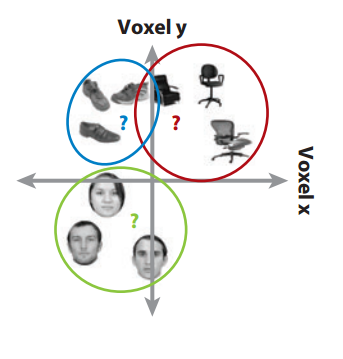
\includegraphics[scale = 0.3]{haxby_example.png}
\end{center}
\begin{itemize}
\item Theory can be extended to handle discrimination between a fixed number of categories
\item Category-based classification is equivalent to a cost function $C(y,y')$ which is equal to 0 if $y$ and $y'$ are from the same category, and 1 otherwise.
\item Sampling of random exemplars is stratified by category, but amounts to a minor adjustment to the variance bounds
\end{itemize}
\end{frame}


\begin{frame}
\frametitle{The end}
\begin{center}
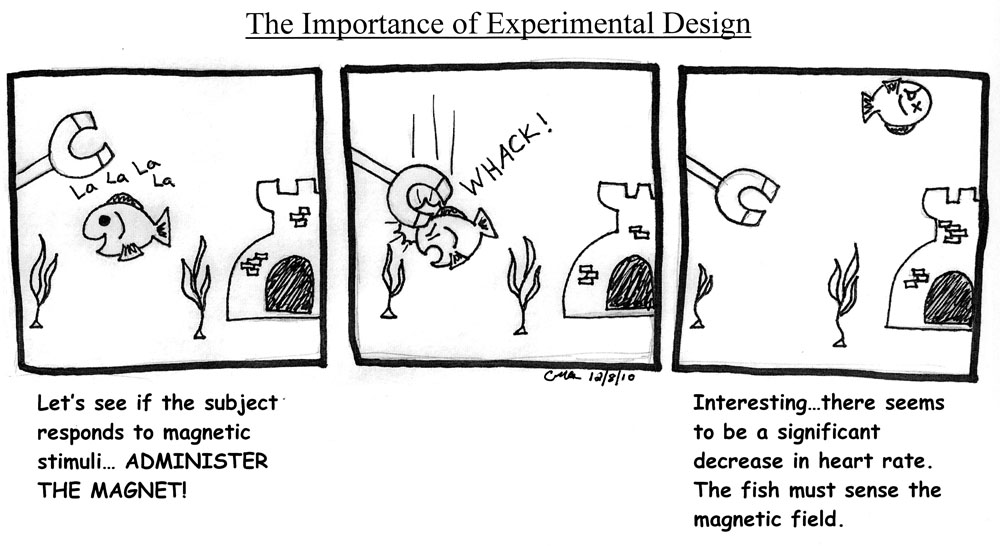
\includegraphics[scale = 1]{c_ambrosino.jpg}


{\tiny(credit C. Ambrosino)}
\end{center}
\end{frame}

\end{document}
